\documentclass[a4paper]{article}
\usepackage[utf8]{inputenc}
\usepackage{authblk}
\usepackage{attrib}
\usepackage{subcaption} % for sugfigures (confusingly!)
\usepackage{graphicx} % for \includegraphics
\usepackage{rotating}
\usepackage{cleveref}

\title{Estimating input-output tables for countries not in the world input--output database}
\author[*]{Thomas P. Ol\'{e}ron Evans}
\author[**]{Robert G. Levy}

\affil[**]{Centre for Advanced Spatial Analysis, UCL Bartlett Faculty of the Built Environment,
90 Tottenham Court Road, London W1T 4TJ, UK}
\affil[*]{Department of Mathematics, University College London, Gower Street, London WC1E 6BT, UK}


\begin{document}
\maketitle

\begin{abstract}
Wow! There's some pretty good stuff in this paper.
\end{abstract}

\section{Analysis}
To check the validity of the estimates, we will now compare the estimated values ``within sample.''
This means comparing the input-output tables of the countries which \textit{are} in WIOD with the estimates for those countries.
\Cref{fig:density} is a great figure. It really shows some great stuff.

\begin{sidewaysfigure}
\centering
\begin{subfigure}{0.49\linewidth}
	\centering
	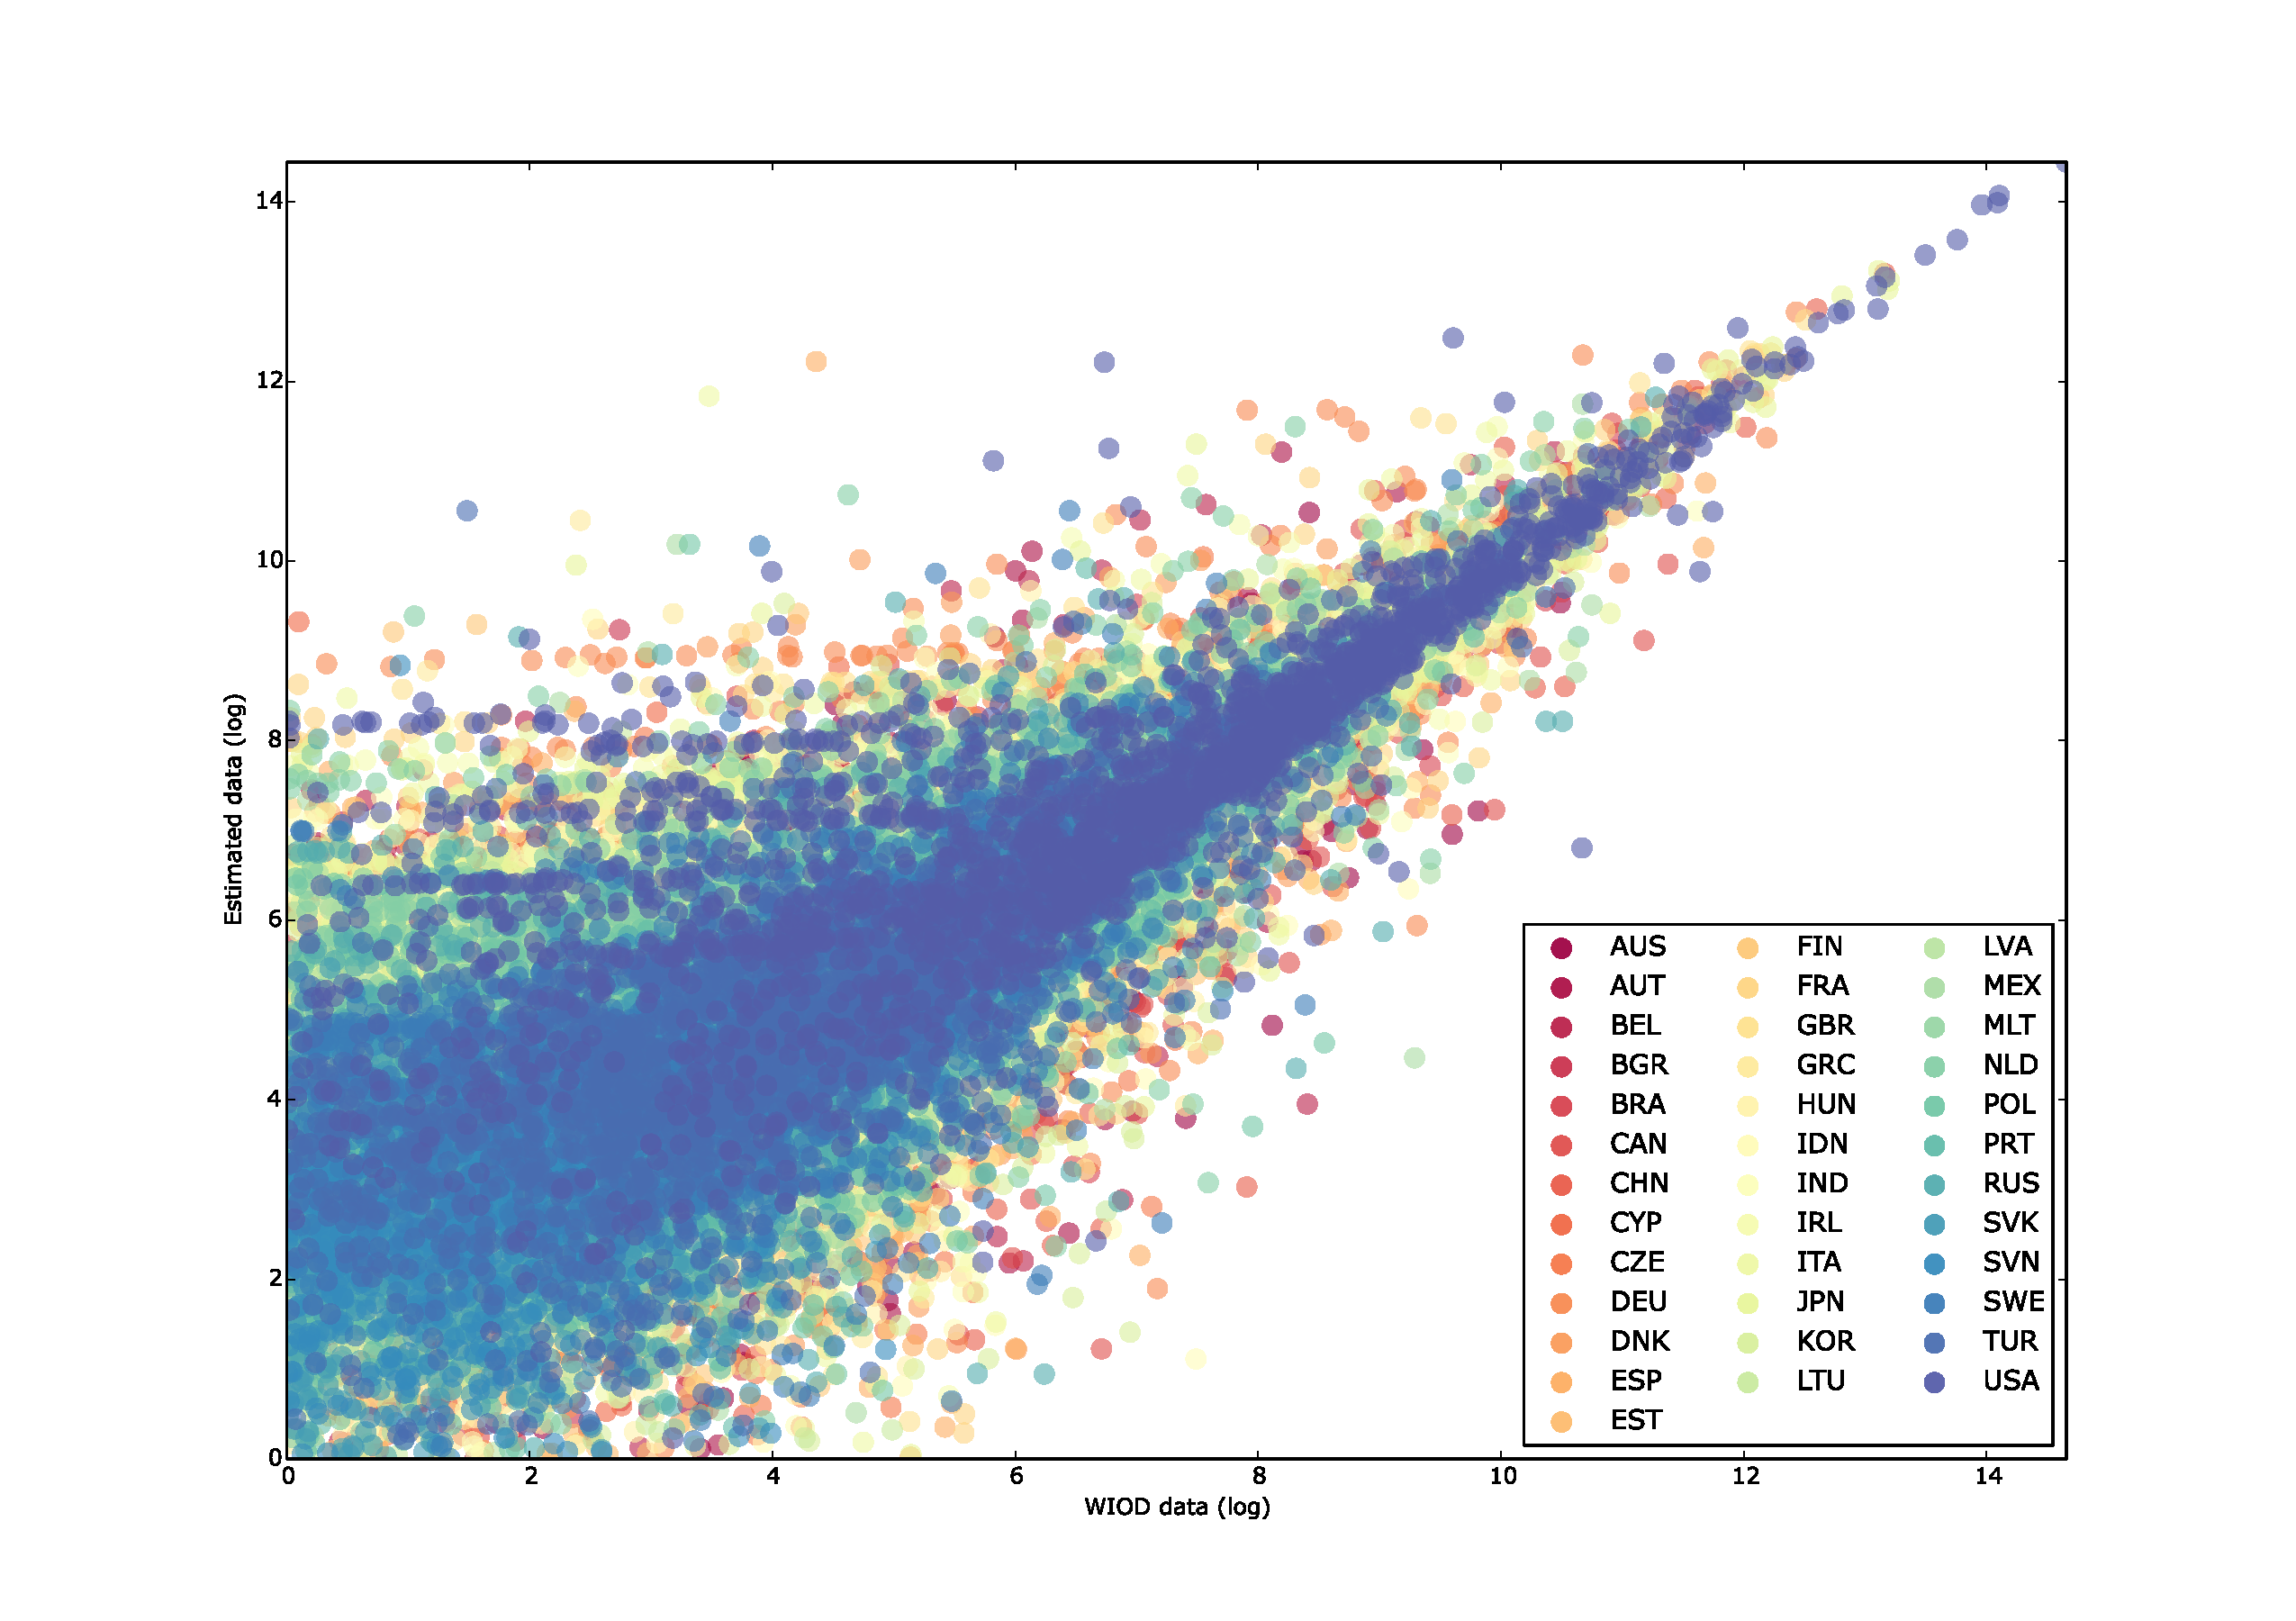
\includegraphics[height=.95\textwidth]{images/est_v_data.png}
	\caption{This one}
	\label{fig:scatter}
\end{subfigure}
\begin{subfigure}{0.49\linewidth}
	\centering
	\includegraphics[height=.95\textwidth]{images/est_v_data_density.png}
	\caption{The other one}
	\label{fig:density}
\end{subfigure}
\end{sidewaysfigure}

\end{document}